\documentclass[a4paper,11pt]{article}
\usepackage[brazil]{babel}
\usepackage[utf8]{inputenc}
\usepackage{amsmath, amssymb}
\usepackage{graphicx}
\usepackage{tikz}
\usepackage{xcolor}
\usepackage{enumitem}
\usepackage{geometry}
\geometry{margin=2cm}
\usepackage{fancyhdr}
\usepackage{pgfplots}
\usepackage{tikz}
\usetikzlibrary{decorations.pathreplacing}
\usepackage{multicol}

% Cores personalizadas
\definecolor{azul25}{RGB}{189,236,241}
\definecolor{azulx2}{RGB}{114,217,228}

\pagestyle{fancy}
\fancyhf{}
\rhead{
\includegraphics[width=3cm]{pei.jpg}}
\lhead{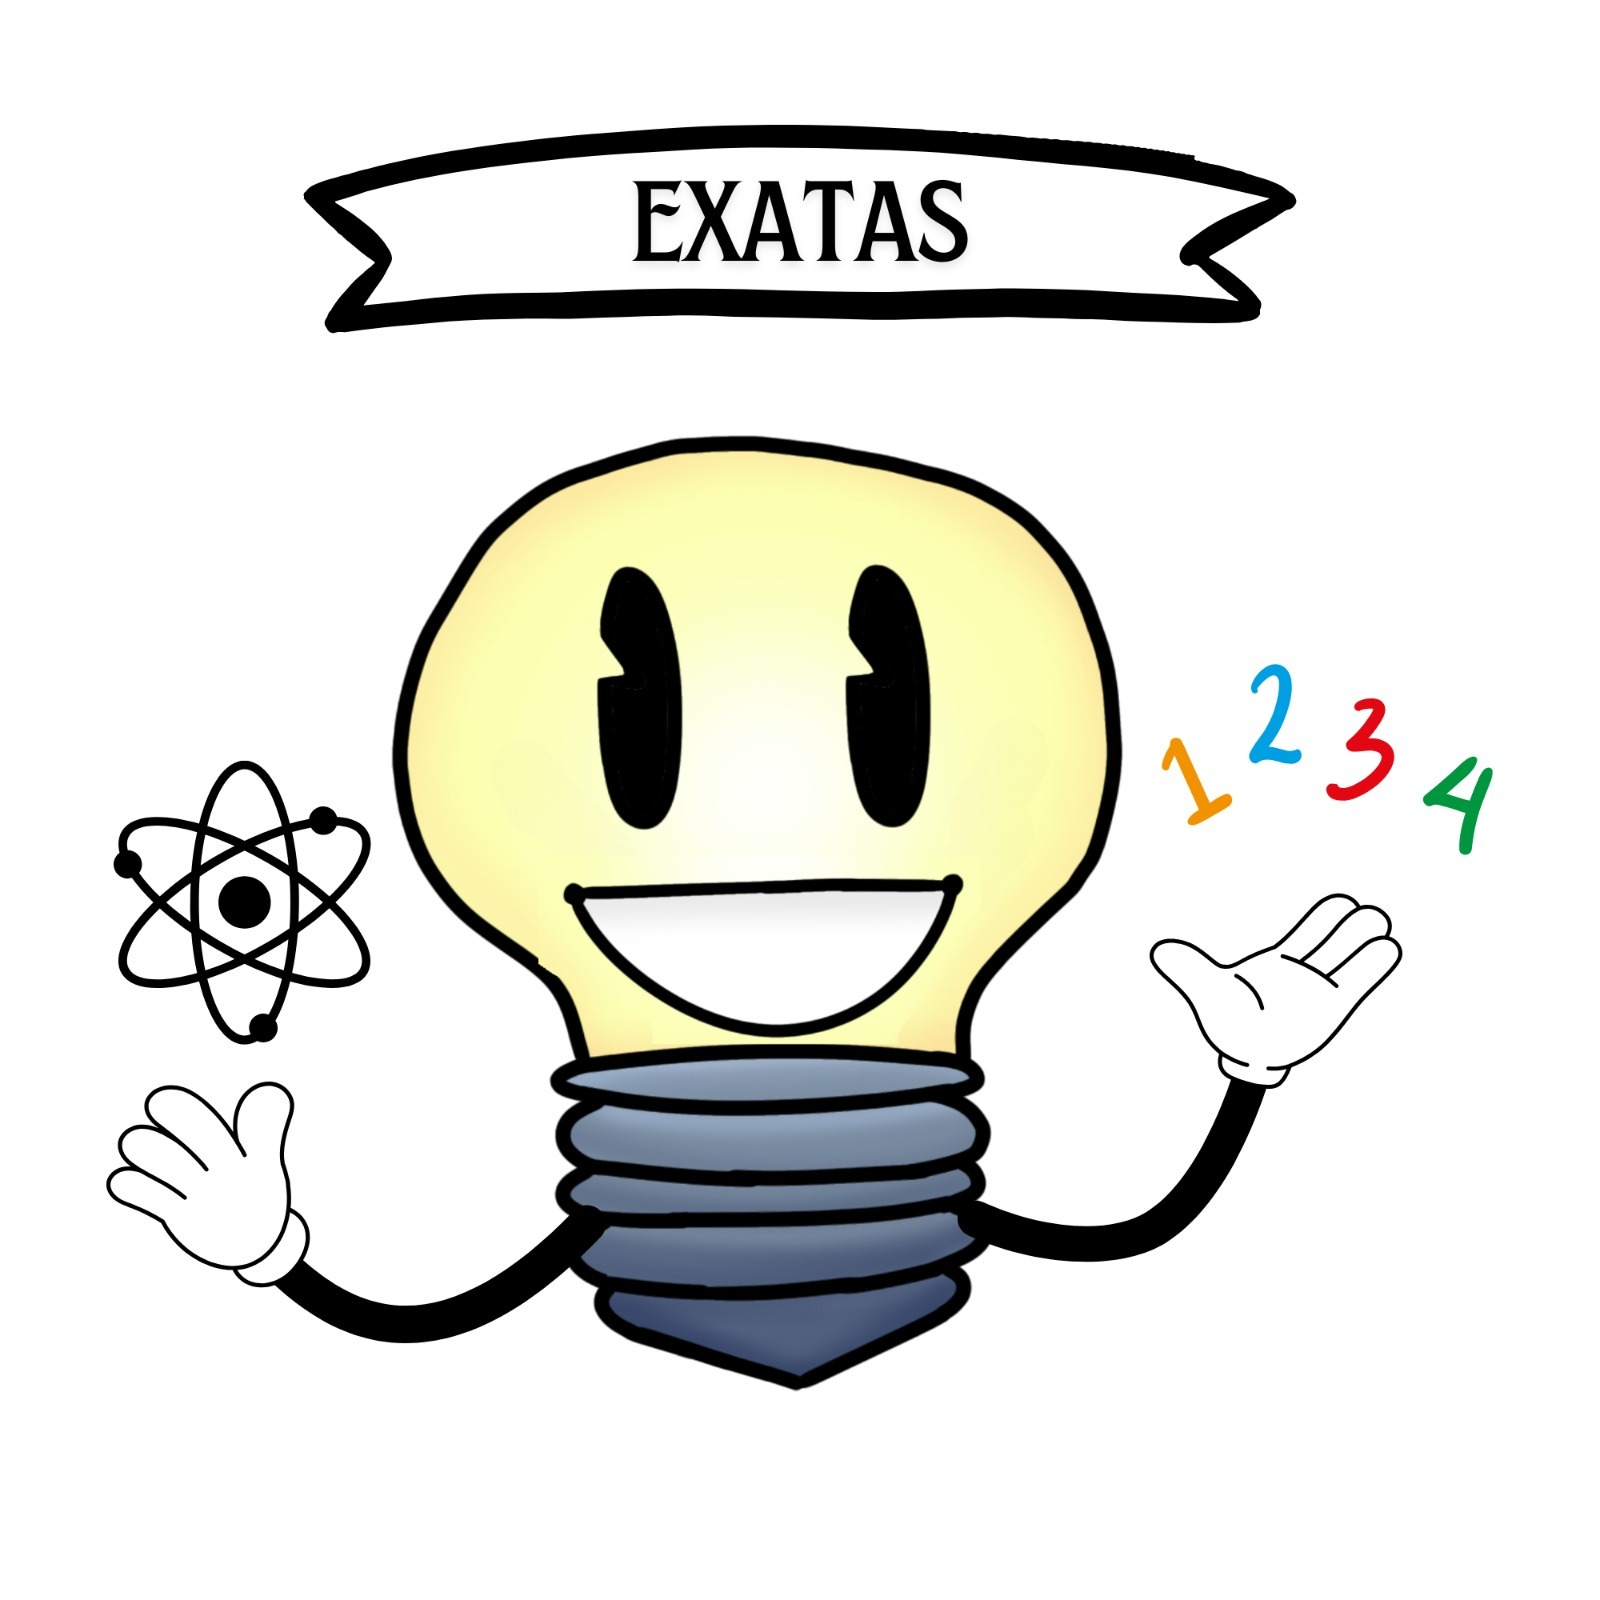
\includegraphics[width=2cm]{exatas.jpg}}
\renewcommand{\headrulewidth}{0pt}

\begin{document}
	
	% Cabeçalho da prova
	\vspace{-1cm}
	\begin{center}
		\textbf{\Large Avaliação de Matemática}\\[0.3cm]
		\begin{tabular}{|p{7cm}|p{4cm}|p{4cm}|}
			\hline
			\textbf{Nome:} & \textbf{Série/Ano:} & \textbf{Data:} \\	
			\hline
			\multicolumn{2}{|l|}{\textbf{Disciplina: Matemática}} & \textbf{Prof.: ISAQUE} \\
			\hline
		\end{tabular}
	\end{center}
	
	\vspace{-0.5cm}
	
	\begin{enumerate}[label=\textbf{\arabic*.}, itemsep=1.2cm]
		
		\item A figura mostra um quadrado \(ABCD\) dividido em quatro partes.
		
		\begin{multicols}{2}
				\begin{center}
				\begin{tikzpicture}[scale=1]
					\fill[azul25] (0,0) rectangle (2.5,2.5);
					\node at (1.25,1.25) {\LARGE 25};
					
					\fill[azulx2] (2.5,2.5) rectangle (4,4);
					\node at (3.25,3.25) {\Large $x^2$};
					
					\draw[thick] (0,0) rectangle (4,4);
					
					\draw[] (0,2.5) -- (4,2.5);			
					\draw[] (2.5,0) -- (2.5,4);
					
					
					
					\foreach \x/\y/\name in {0/4/A, 0/0/B, 4/0/C, 4/4/D}
					\filldraw[purple] (0,4) circle (2pt) node[anchor=east] {\textbf{A}};
					\filldraw[purple] (0,0) circle (2pt) node[anchor=east] {\textbf{B}};
					\filldraw[purple] (4,0) circle (2pt) node[anchor=west] {\textbf{C}};
					\filldraw[purple] (4,4) circle (2pt) node[anchor=west] {\textbf{D}};
					
				\end{tikzpicture}
			\end{center}
			
			As partes destacadas em azul também são quadrados, cujas
			medidas de superfície, em unidades de área (u.a.), estão indicadas na figura.
			
			\begin{enumerate}
				\item[a)] Determine a expressão algébrica que representa a medida dos lados do quadrado \(ABCD\).
				\item[b)] Encontre a expressão algébrica que representa a área do quadrado \(ABCD\).
			\end{enumerate}
		\end{multicols}
		
		\vspace{-1.5cm}	
		
		\item Escreva a expressão algébrica que representa a área e o perímetro da seguinte figura:
		\begin{multicols}{2}
				\begin{center}
				\begin{tikzpicture}[scale=0.4]
					\coordinate (A) at (0,0);
					\coordinate (B) at (0,6);
					\coordinate (C) at (4,6);
					\coordinate (D) at (8,0);
					\draw [thick] (A) -- (B) -- (C) -- (D) -- (A);
					\draw [decorate,decoration={brace,amplitude=8pt}] (A) -- (B) node[midway,left=8pt] {\small 6};
					\draw [decorate,decoration={brace,amplitude=8pt}] (B) -- (C) node[midway,above=8pt] {\small $x$};
					\draw [decorate,decoration={brace,amplitude=8pt}] (C) -- (D) node[midway,right=8pt] {\small $y$};
					\draw [decorate,decoration={brace,mirror,amplitude=8pt}] (A) -- (D) node[midway,below=8pt] {\small $x+8$};
				\end{tikzpicture}
			\end{center}
			
			Calcule o valor da área e do perímetro quando \(x=3\) e \(y=10\).
		\end{multicols}
		
		\vspace{-1.5cm}
	
		\item A Câmara Municipal de Araraquara está realizando um estudo sobre o impacto ambiental de ações urbanas, utilizando um modelo matemático para avaliar a eficiência de iniciativas de sustentabilidade. O índice de impacto ambiental \(y\) é calculado pela fórmula:
		
		\[
		y = \frac{0{,}49 - x^2}{0{,}7 + x}
		\]
		
		onde \(x\) representa um parâmetro relacionado à quantidade de resíduos gerados em toneladas. Tendo em vista que em determinado cenário o valor de \(x = 1{,}3\), qual é o índice de impacto ambiental \(y\)?
		
		\vspace{-1.3cm}
		
		\item Um estudante de química está preparando uma mistura que apresentará em um trabalho, mas derramou um produto sobre seu caderno e suas anotações foram parcialmente apagadas. Sabe-se que precisa misturar \(x\) ml de um produto chamado de A com o triplo dessa quantidade de outro chamado de B e adicionar mais 50 ml de um ingrediente secreto. Se no final a mistura completa terá 290 ml, escreva a equação que permite descobrir corretamente a quantidade \(x\) do produto A.
		
		\vspace{-1.3cm}
		
		\item Simplifique as expressões:
		
		\begin{multicols}{3}
				\begin{enumerate}[label=\alph*)]
				\item \(x + x\)
				\item \(x \cdot x\)
				\item \(2x + 3x\)
				\item \(2x \cdot 3x\)
				\item \((x + 3)(x + 2)\)
				\item \((x + 3)^2\)
				\item \((x - 3)^2\)
			\end{enumerate}
		\end{multicols}
	
		
	\end{enumerate}
	
\end{document}
